\pagestyle{fancy}
\normalsize
\linespread{1.5}\selectfont
\label{mark:chapter3}\chapter{轻量级重组糖算法}
\addtocontents{los}{\protect\addvspace{10pt}}

\section{对语言的规定}

\subsection{文法限制}
首先,我们需要将整个语言限定在基于树形表达式的结构化语言。

\newtheorem*{Def}{定义}

\label{mark:struct}\begin{Def}[结构化]
	对于每个表达式中的子表达式,其规约规则只和子表达式本身有关。
\end{Def}

此限制约束了Corelang的作用域,限制语言子表达式不能有对外的副作用。我们将在第五章详细讨论副作用的一些具体解决办法。

\begin{Def}[树形表达式]
	此处我们使用类似Lisp的S表达式的递归树,基础定义如下
\end{Def}

\[
\begin{array}{rcl}
\mbox{Exp} &::=& (\mbox{Headid}~\mbox{Exp}*)\\
&|& \mbox{Value}\\
&|& \mbox{Variable}
\end{array}
\]

\subsection{上下文规则限制}


对每个子表达式都是CoreLang表达式的表达式Exp,最多只能有一条规约路径(通过求值顺序约束)。这一点约束并不过分,为了保证每个程序只能有一条执行路径。

对SurfLang,任意一个语法糖只能有一个CoreLang的表达式与之对应。这也是很自然的要求,因为同一个语法糖不应该有二义性。对于求值顺序,SurfLang上的子表达式约定类似完全规约的规则,任何子表达式都可以首先进行规约。

\subsection{语法糖形式限制}

对于语法糖的形式限制为如下。

\fbox{
$(\mbox{Surfid}\;e_{1}\;e_{2}\;\ldots)→(Headid\; \ldots)$
}

其中的主要约束是在语法糖这一侧不能出现形如$(\mbox{Surfid}\;\ldots\;(e1\;e2)\ldots))$这种形式。这对语法糖的表达能力并不会造成影响。\footnote{此约束主要是为了算法描述和实现更简单。}

\subsection{文法描述}
在PLT Redex中,我们将CoreLang和SurfLang视为同一个语言。则当我们定义了一个语言内部各种规约规则后,对于任意Exp都有其对应的一条或多条规约规则。根据对CoreLang的约定,有多条规约规则的表达式必然存在SurfLang的表达式。

为了区分CoreLang的语言和SurfLang的语言,我们将表达式的文法定义为如下
\begin{center}
	\framebox[35em][l]{
	\parbox[t]{35em}{
		\[
		\begin{array}{rcl}
		\mbox{Exp} &::=& \mbox{Coreexp}\\
		&|& \mbox{Surfexp}\\
		&|& \mbox{Commonexp}\\
		&|& \mbox{OtherSurfexp}\\
		&|& \mbox{OtherCommonexp}
		\end{array}
		\]
		
		\[
		\begin{array}{rcl}
		\mbox{Coreexp} &::=& (\mbox{CoreHead}~\mbox{Exp}*)
		\end{array}
		\]
		
		\[
		\begin{array}{rcl}
		\mbox{Surfexp} &::=& (\mbox{SurfHead}~(\mbox{Surfexp}~|~\mbox{Commonexp})*)
		\end{array}
		\]
		
		\[
		\begin{array}{rcl}
		\mbox{Commonexp} &::=& (\mbox{CommonHead}~(\mbox{Surfexp}~|~\mbox{Commonexp})*)\\
		&|& \mbox{Value}\\
		&|& \mbox{Variable}
		\end{array}
		\]
		
		\[
		\begin{array}{rcl}
		\mbox{OtherSurfexp} &::=& (\mbox{SurfHead}~\mbox{Exp}*~\mbox{Coreexp}~\mbox{Exp}*)
		\end{array}
		\]
		
		\[
		\begin{array}{rcl}
		\mbox{OtherCommonexp} &::=& (\mbox{CommonHead}~\mbox{Exp}*~\mbox{Coreexp}~\mbox{Exp}*)
		\end{array}
		\]
	}
}
\end{center}




在这里,我们将CoreLang的表达式一部分提取处理作为公共表达式,是因为在重组糖序列中必定有一些表达式是属于CoreLang的,但需要在序列中输出(比如说数字,布尔表达式,以及一些可能的基础运算)。在这种情况下,对于Commonexp来说,满足CoreLang的约束,但是也可以作为重组糖的中间序列输出

可以看出,在我们的重组糖方法中,可以输出的表达式是Surfexp和Commonexp,即不存在任何子表达式中存在Coreexp。


\section{算法描述}
本节讨论建立在符合约定的语言基础上。

\subsection{核心算法}

{\bfseries 核心算法f}\footnote{核心思想:对于每个表达式Exp,我们将对它所有规约规则中选择一条符合resugaring的仿真性规则的规约,且尽可能不破坏任何语法糖。}定义如下图\ref{fig:corealgo}:(输入为一个任意Exp,输出为应用应该执行的规约规则后的表达式)

\begin{figure}[ht]
	\centering
	\framebox[35em][l]{
		\parbox{\textwidth}{
			$f$($Exp$): \qquad \qquad \qquad \qquad \qquad \qquad \quad //$Exp$=$(Headid~Subexp_{1}~\ldots~Subexp_{\ldots})$
			
			\qquad Let $ListofExp'~=~\{Exp'_{1}\;,Exp'_{2}~\ldots\}$
			
			\qquad if (Exp is Coreexp or Commonexp or OtherCommonexp):
			
			\qquad \qquad if (Lengthof ($ListofExp'$) == 0): \qquad \qquad \qquad \qquad \qquad \qquad //$Rule1.3$
			
			\qquad \qquad \qquad return null;
			
			\qquad \qquad else if (Lengthof ($ListofExp'$) == 1): \qquad \qquad \qquad \qquad \qquad //$Rule1.1$
			
			\qquad \qquad \qquad return first($ListofExp'$);
			
			\qquad \qquad else:
			
			\qquad \qquad \qquad return $Exp'_{i}$ = $(Headid~Subexp_{1}~\ldots~Subexp'_{i}~\ldots)$; \qquad  ~//$Rule1.2$ 
			
			/*where i is the index of subexp which have to be reduced. */
			
			\qquad else if (Exp is Surfexp or OtherSurfexp):
			
			\qquad \qquad if (Exp have to be desugared): \qquad \qquad \qquad \qquad \qquad \qquad \quad ~//$Rule2.1$
			
			\qquad \qquad \qquad return desugarsurf(Exp);
			
			\qquad \qquad else: let DesugarExp' = desugarsurf(Exp): \qquad \qquad \qquad \qquad  ~//$Rule2.2$

			
			\qquad \qquad \qquad if ($Subexp_{i}$ is reduced to $Subexp'_{i}$ during $f(DesugarExp')$):
			
			\qquad \qquad \qquad \qquad return $Exp'_{i}$ = $(Headid~Subexp_{1}~\ldots~Subexp'_{i}~\ldots)$;  //$Rule2.2.1$
			
			\qquad \qquad \qquad else:
			
			\qquad \qquad \qquad \qquad return desugarsurf(Exp); \qquad \qquad \qquad \qquad \qquad  ~~~//$Rule2.2.2$
		}
	}
\caption{核心算法f}
\label{fig:corealgo}
\end{figure}

接下来对整个算法语言说明,分别解释每一个分支规则。

对Exp尝试所有规约规则,得到多个可能的表达式ListofExp'=\{$Exp'_{1}$,$Exp'_{2}$,$\ldots$\}

\begin{flushleft}
	\large{\bfseries{
			如果Exp是Coreexp或Commonexp或OtherCommonexp,则其规约规则	
		}	
	}	
\end{flushleft}
\begin{itemize}
	\item 或是将表达式规约到另一个表达式,此时只有一条规则,应用后输出Exp';
	
	($Rule1.1$)
	\item 或是其规约不满足导致内部子表达式需要规约,此时因为CoreLang的定序性,只会有一个子表达式被规约(且此表达式为Surfexp),此时对该子表达式Subexp递归调用核心算法f得到Subexp’,则在ListofExp'中找到将此Exp中子表达式Subexp规约为Subexp’的表达式就是我们需要的表达式;($Rule1.2$)
	\item 或是已经无法被规约(ListofExp'为空),此时返回的表达式为空。($Rule1.3$)
\end{itemize}

\begin{flushleft}
	\large{\bfseries{
			如果Exp是Surfexp或OtherSurfexp	
		}
	}
\end{flushleft}
\begin{itemize}
	\item 如果内部子表达式无可规约的,则必然会展开该语法糖,此时输出表达式为Exp解糖后的表达式;($Rule2.1$)
	\item 如果存在可规约的子表达式对于每个子表达式,如果可规约,则根据我们的设定,存在一条关于此子表达式的规约规则。因此每个子表达式都可能被规约的前提下,我们需要对Surfexp或OtherSurfexp的外层语法糖进行展开为DesugarExp’(此展开只有一种规约规则对应),之后对Exp’调用核心算法f({\bfseries 单步尝试})
	\begin{itemize}
		\item 如果f(DesugarExp')是对DesugarExp'的子表达式进行规约,由于此子表达式一定由Exp的子表达式组成,需要检测是哪一个子表达式$Subexp_{i}$先被规约为$Subexp'_{i}$,则在ListofExp'中将此子表达式规约的表达式就是所需要的。($Rule2.2.1$)
		\item 如果f(DesugarExp')不是对子表达式进行规约,则说明这个糖不会被重组(此糖被展开后必然会被继续破坏),因此输出不在ListofExp'中,而是输出DesugarExp'
			($Rule2.2.2$)
	\end{itemize}
\end{itemize}

\subsection{轻量级重组糖算法}

{\bfseries 整体算法lightweight-resugaring}定义如下图\ref{fig:lwresugar}。

算法Lightweight-resugaring:给定Surfexp的表达式$Exp$,输出其重组糖序列\\
\begin{figure}[h]
	\centering
	\framebox[35em][l]{
		\parbox{\textwidth}{
			$Lightweight-resugaring$($Exp$)
			
			\qquad while ($tmpexp$ == f($Exp$)))
			
			\qquad \qquad if ($tmpexp$ is empty):
			
			\qquad \qquad \qquad return;
			
			\qquad \qquad else if ($tmpexp$ is surfexp or commonexp):
			
			\qquad \qquad \qquad output $tmpexp$;
			
			\qquad \qquad \qquad $Lightweight-resugaring$($tmpexp$);
			
			\qquad \qquad else:
			
			\qquad \qquad \qquad $Lightweight-resugaring$($tmpexp$);
		}
	}
\caption{整体算法}
\label{fig:lwresugar}
\end{figure}


\section{正确性证明}

首先,由于我们的算法和先解糖后重组糖的区别就是我们只在需要的时候将语法糖解开,而传统意义上语法糖是先将语法糖全部展开然后再CoreLang上进行执行。

其次,为了证明方便,定义一些术语。

$(Headid\;Subexp_{1}\;Subexp_{\ldots} \ldots)$为任意可规约表达式

对表达式运用Headid的对应规则进行规约,称为外部规约。

对其子表达式$Subexp_{i}$规约。其中$Subexp_{i}$为$(Headid_{i}~Subexp_{i1}~Subexp_{i\ldots} \ldots)$
\begin{itemize}
	\item 如果对$Subexp_{i}$ = $(Headid_{i}~Subexp_{i1}~Subexp_{i\ldots} \ldots)$进行外部规约,则称为表面规约。
	\item 如果对$Subexp_{ij}$进行规约,则称为内部规约。
\end{itemize}

{\bfseries 例:}

$(\mbox{if}\; \#t\; Exp_{1}\; Exp_{2})$--->$Exp1$ \begin{flushright}外部规约\end{flushright}

$(\mbox{if}\; (\mbox{And}\; \#t\; \#f)\; Exp_{1}\; Exp_{2})$--->$(\mbox{if}\; (\mbox{if}\; \#t\; \#f\; \#f)\; Exp_{1}\; Exp_{2})$ \begin{flushright}表面规约\end{flushright}

$(\mbox{if}\; (\mbox{And}\; (\mbox{And}\; \#t\; \#t)\; \#t)\; \#f)\; Exp_{1}\; Exp_{2})$--->$(\mbox{if}\; (\mbox{And}\; \#t\; \#t)\; Exp_{1}\; Exp_{2})$ \begin{flushright}内部规约\end{flushright}

对$Exp$=$(Headid\;Subexp_{1}\;Subexp_{\ldots} \ldots)$,$Exp$称为上层表达式,$Subexp_{i}$称为下层表达式。

%定理 证明
\subsection{仿真性}
仿真性:求值序列需要和在CoreLang上的求值顺序相同,即存在CoreLang上的求值序列中的部分中间过程与该序列中的元素对应。

\newtheorem{mythm}{定理}[section]
\begin{mythm}[仿真性]
	我们的轻量级重组糖具有仿真性。
\end{mythm}
\begin{proof}[仿真性证明]
	对核心算法f逐条进行分析。
	
	首先$Rule1.1$和$Rule1.3$不会影响仿真性,因为其本身就是在对CoreLang的表达式进行操作;
	
	对$Rule1.2$是对子表达式进行规约(用核心算法f),因为$Coreexp$内部的上下文规则是定的,因此即使将表达式所有糖都进行展开,也是该位置先进行规约。而在递归调用f的过程中,由于表达式深度优先,如果对下层的表达式调用f满足仿真性,那么此处上层表达式也满足仿真性。
	
	对$Rule2.1$和$Rule2.2.2$,解糖操作也不会破坏仿真性。
	
	对$Rule2.2.1$,由于仿真性的定义,重组糖的序列的每一步可以解糖到CoreLang上执行序列的步骤,因此证明仿真性只需要证明我们的序列在CoreLang上的序列有对应。我们在对$(Surfid\;Subexp_{1}\;Subexp_{\ldots}\;\ldots)$进行正常运算时,也会将其依据Surfid的规约规则进行展开;而在我们的核心算法中,我们也是这样进行单步展开,区别在于内部的糖没有规约。由于Rule2.2对Exp进行外部规约后得到DesugarExp',并调用了f(DesugarExp')
	\begin{itemize}
		\item 如果DesugarExp'是$Coreexp$或$Commonexp$或$OtherCommonexp$,且其子表达式规约,因此对于将Exp完全解糖后也是该子表达式的位置进行规约,其他子表达式的内容不变,因此对Exp的该子表达式规约后完全解糖和对Exp整体先解糖再规约,得到的是相同的表达式。如下图\ref{fig:emulation}所示
		
		\begin{figure}[h]
			\centering
			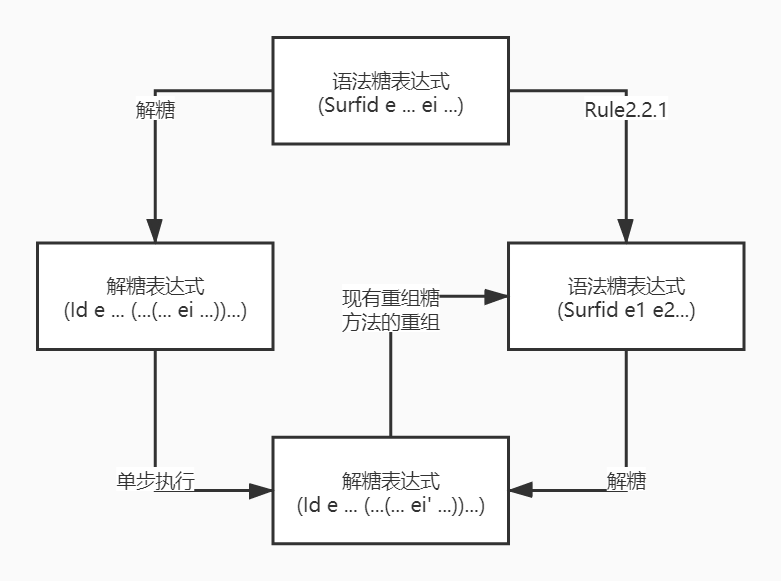
\includegraphics[width=12cm]{images/chapter3/flowgraph.jpg}
			\caption{Rule2.2.1仿真性图示}
			\label{fig:emulation}
		\end{figure}
		
		\item 如果DesugarExp'是$Surfexp$或$OtherSurfexp$,则此处将递归调用f,由于表达式深度有限,如果下层的表达式满足仿真性,则此处也满足仿真性.
	\end{itemize}

证毕。

\end{proof}






%如果被规约的子表达式是$Coreexp$或$Commonexp$,则和CoreLang上的表现一致;如果是$Surfexp$或$OtherSurfexp$,则相当于一个解糖操作,解糖是不影响仿真性的;而如果是




\subsection{抽象性}
抽象性:求值序列中只存在SurfLang中存在的术语,没有引入CoreLang中的术语。

抽象性的正确性是显然的,因为我们在每次输出都判断了输出的$Exp$是否是$Surfexp$或$Commonexp$。(在lightweight-resugaring算法中)

\subsection{覆盖性}
覆盖性:在求值序列中没有跳过一些中间过程。

\newtheorem{lemma}{引理}[section]

\begin{lemma}
	如果在重组糖序列中语法糖没有在不必须破坏的时候被破坏,那么就没有跳过中间过程。
\end{lemma}

\begin{proof}[引理证明]
	假设没有语法糖提前破坏的情况下,存在CoreLang序列中的某一项
	
	$Exp$=$(Headid\;Subexp_{1}\;Subexp_{\ldots} \ldots)$可被重组为
	
	$ResugarExp'$=$(Surfid\;Subexp'_{1}\;Subexp'_{\ldots}\ldots)$,且没有在算法lightweight-resugaring中被表现。则说明
	\begin{itemize}
		\item 或是重组糖序列中存在
		
		$ResugarExp$=$(Surfid\;Subexp'_{1}\;\ldots\;Subexp_{i}\;Subexp'_{\ldots}\ldots)$
		
		使得$ResugarExp$解糖后得到的表达式单步规约得到$Exp$,且此时该单步规约将$ResugarExp$中子表达式$Subexp_{i}$对应部分规约。我们发现此时$ResugarExp$的语法糖结构并没有被破坏,因此如果不能展示$ResugarExp'$则是提前破坏了不必要破坏的语法糖,与假设前提矛盾。
		
		\item 或是重组糖序列中存在
		
		$ResugarExp$=$(Surfid'\;\ldots\;ResugarExp'\;\ldots)$
		
		使得$ResugarExp$解糖后得到的表达式单步规约得到$Exp$,且该$Exp$是从$ResugarExp$中的子表达式$ResugarExp'$解糖得到,说明此步单步规约不涉及$ResugarExp'$的规约。而如果不能展示$ResugarExp'$,则说明该语法糖在执行前面的序列被提前破坏了,也与假设矛盾。

	\end{itemize}

证毕。
\end{proof}

\begin{mythm}[覆盖性]
	我们的轻量级重组糖具有覆盖性。
\end{mythm}

\begin{proof}
	由引理可知,只需证明核心算法f得每一条都不会将语法糖在不必要破坏时被破坏。
	对f的每一条进行讨论。
	
	对Rule1.1和Rule1.3显然没有破坏不必须破坏的语法糖。
	
	对Rule1.2,由于CoreLang的表达式需要进一步规约必须对特定子表达式进行规约,因此要对相应的下层表达式作用f。同仿真性,由于表达式深度有限,下层表达式作用f满足覆盖性可递归证明上层表达式满足覆盖性。
	
	对Rule2.1,此时必须破坏语法糖,否则无法继续规约,因此页没有破坏不必须破坏的语法糖。
	
	对Rule2.2.1,与Rule1.2相同,递归的对下层表达式作用f,递归证明覆盖性。
	
	对Rule2.2.2,因为单步尝试后发现语法糖解糖后,解糖后结构继续被破坏,因此无法还原回语法糖,也是必须破坏的语法糖。
	
	因此求值序列没有破坏任何不必须破坏的语法糖,核心算法f满足覆盖性。
\end{proof}



